%!TEX root = ../thesis.tex
\chapter{Background}

Dynamic mapping is becoming an increasingly important requirement for digital musical instruments. This chapter surveys currently available tools that allow for manipulation of musical and non-musical networks in real time. The first section presents a review of mapping itself, both from a theoretical and a musical standpoint. This portion also introduces the libmapper application programming interface. The second section reviews relevant work in the visual representation of information. The following portion describes applicable techniques in user interface design. Finally, a review of user interfaces for mapping is presented.

%%%%%%%%%%%%%%%%%%%%%%%%%%%%%%%%%%%%%%%%%%%%%%%%%%%%%%%%%%%%%%%%%%%%%%%%%%%%%%%%%%%%%%%%%%%%%%%%%%%%%%%%%%%%%%%%%%%%%%%%%%%%%%%%%%%%%%%%%%%%%%%%%%%%%%%%%%%%%%%%%%%%%%%%%%%%%%%%%%%%%%%%%%%%%%%%%%%%%%%%%%%%%%%%%%%%%%%%%%%%%%%%%%%%%%%%%%%%%%%%%%%%%%%%%%%%%%%%%%%%%%%%%%%%%%%%%%%%%%%%%%%%%%%%%%%%
			\section{Mapping}

At the most fundamental level, \emph{mapping} is the act of associating two or more sets of information. Mappings can be mathematical, computational, linguistic (like translation), geographic, or even poetic\footnote{What is metaphor if not the association of unlike things?}. Within the context of DMI design mapping is the relationship between sensor outputs and synthesis inputs. The entire character of a new instrument can be drastically altered though mapping, even while control surface and sound source are held constant \shortcite{hunt_mapping_is_important}. As a result, the theoretical formalism of mapping becomes yet another necessary tool in the modern instrument designer's arsenal.

%%%%%%%%%%%%%%%%%%%%%%%%%%%%%%%%%%%%%%%%%%%%%%%%%%%%%%%%%%%%%%%%%%%%%%%%%%%%%%%%%%%%%%%%%%%%%%%%%%%%%%%%%%%%%%%%%%%%%%%%%%%%%%%%%%%%%%%%%%%%%%%%%%
	\subsection{Mapping Theory}

\subsubsection{Mapping as function and mapping cardinality}
\label{sec:mapping_classes}

From the perspective of mathematics, the term \emph{mapping} is very nearly synonymous with \emph{function} \cite{native_set_theory}, as both describe how one set of numbers corresponds with another. The first group is commonly referred to as the \emph{domain} and the second as the \emph{codomain} or \emph{range}. An in-depth review of functions in mathematics is beyond the scope of this thesis, however a few fundamental examples will be useful for reference in section \ref{sec:mappingforDMIs}. The following are instances of two basic types of mathematical functions:

\begin{equation} y = 2x - 1 \label{eq:one-to-one} \end{equation} 
\begin{equation} y = x^2  \label{eq:many-to-one}  \end{equation}

Each function takes a single input value (\emph{x}) and \emph{maps} that number onto its range (\emph{y}). 
%For example, an input of \textbf{5} maps to \textbf{9} in equation \ref{eq:one-to-one}, while the same input results in an output \textbf{25} for equation \ref{eq:one-to-many}. 
The fact that each of these equations take in only a single number as input, and output a single number in turn, means they can be graphed in a two dimensional space. This is not necessarily the case, as functions can input and output lists of numbers (vectors). Mathematically they are not very interesting, but they represent two fundamentally different \emph{kinds} of functions.

\begin{figure}[h]
	\centering
	\begin{tikzpicture}
		\begin{axis}[my style, xtick={-2,-1,...,2}, ytick={-2,-1,...,2}, xmin=-2, xmax=2, ymin=-2, ymax=3]
			\addplot[domain=-100:100]{2*x-1}; 
		\end{axis}
	\end{tikzpicture}	
\caption{The function described in equation \ref{eq:one-to-one}, graphed in two dimensions.}
\label{fig:one-to-one_graph}
\end{figure}

For equation \ref{eq:one-to-one} each input value has \emph{one and only one} corresponding output value. The same is true if the function is to be inverted, as each output value corresponds to only one input value. The range is simply a scaled and shifted version of the domain. The mapping's \emph{one-to-one} nature can clearly be seen in figure \ref{fig:one-to-one_graph}. To mathematicians this is known as the mapping's \emph{cardinality}.

\begin{figure}[h]
	\centering
	\begin{tikzpicture}
		\begin{axis}[my style, xtick={-3,-2,...,3}, ytick={-3,-2,...,3}, xmin=-3, xmax=3, ymin=-1, ymax=4]
			\addplot[domain=-3:3]{x^2}; 
		\end{axis}
	\end{tikzpicture}
\caption{Equation \ref{eq:many-to-one} projected on the Cartesian plane.}
\label{fig:many-to-one_graph}
\end{figure}

This is not the case for equation \ref{eq:many-to-one}, for although each input has only one output, single positions in the codomain can have multiple corresponding inputs (e.g. both $3^2$ \emph{and} $-3^2$ are equal to 9). Thus we can consider equation \ref{eq:many-to-one} to be a classical example of a mapping with a cardinality \emph{many-to-one}. In figure \ref{fig:many-to-one_graph} the range of the function is wrapped back onto itself such that a horizontal line could intersect the curve twice.

Two more mapping cardinalities are relevant to instrument design, an example of each:  

\begin{equation} y = \pm\sqrt{x} \label{eq:one-to-many} \end{equation} 
\begin{equation} y = \pm\sqrt{1 - x^2} \label{eq:many-to-many} \end{equation} 

They are not considered to be functions by mathematicians\footnote{In mathematics, a true function can have no more than one output value for every input value.}, but are nonetheless important for our purposes. In equation \ref{eq:one-to-many} a single input can result in multiple outputs (an input of 4 results in the output of \emph{both} 2 and -2), yet each output has only a single input. This is simply the inverse function of equation \ref{eq:many-to-one}, and is an example of a \emph{one-to-many} mapping. On a graph of such a mapping, a \emph{vertical} line may cross at multiple points. The final equation is that of a circle centered at the origin with a radius of one. This is a \emph{many-to-many} mapping, as both it an its inverse result in multiple outputs from a single input.

\begin{figure}[ht]
	\centering
	\begin{tikzpicture}
		\begin{axis}[my style, xtick={-1,...,1}, ytick={-1,...,1}, xmin=-1.5, xmax=1.5, ymin=-1.5, ymax=1.5]
			\addplot[domain=-1:1]{sqrt(1 - x^2)}; 
			\addplot[domain=-1:1]{-sqrt(1 - x^2)}; 
		\end{axis}
	\end{tikzpicture}
\caption{Equation \ref{eq:many-to-many}, a many-to-many mapping.}
\end{figure}

Though a graphical plane is the most common way for mathematicians to visualize two-dimensional functions, drawing the direct association between input and output will be more useful going forward. Figure \ref{fig:types_of_mapping} provides an illustration of such an approach. The astute reader will notice a striking similarity to the GUI view mode described in section \ref{sec:list_view} and these diagrams.  

\begin{figure}[ht]
\centering
	\scalebox{1}{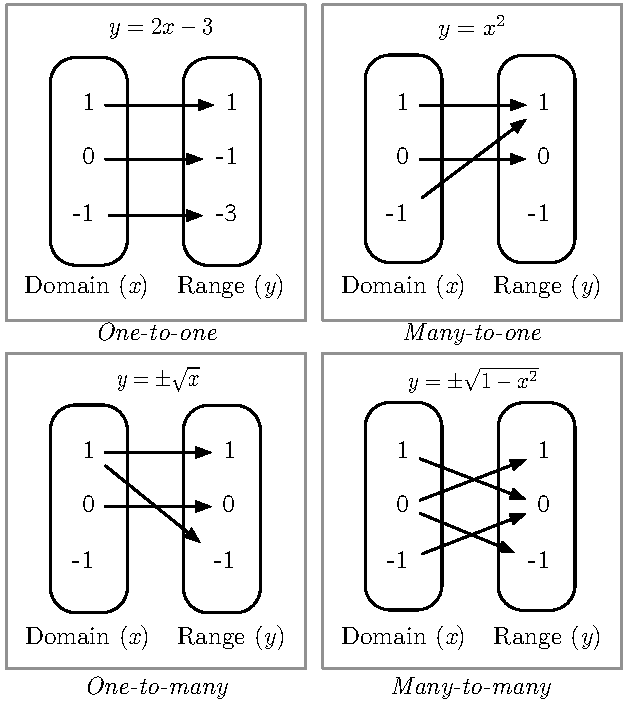
\includegraphics{figures/types_of_mapping}}
\caption{The four mapping classes}
\label{fig:types_of_mapping}
\end{figure}

	\subsubsection{Mapping as association}

In computer science, a mapping is less commonly referred to as a function and more usually called an \emph{associative array} or a \emph{dictionary}, though the word \emph{map} is also used \cite{data_structures}. This type of data structure\footnote{What computer scientist call particular ways of storing and organizing data.} is generally the most flexible way for computers store information. An associative array consists of key/value pairs, where the \emph{value} is the data to be stored and the \emph{key} is the reference to that data. 

\begin{table}
\centering
\Tcaption{An example of key/value pairs (contries and currencies)}
\label{tab:key_value_pairs}
\begin{tabular}{l l}
\hline\hline
key&value\\
\hline
Canada&Dollar\\
France&Euro\\
Bahrain&Dinar\\
Germany&Euro\\
Angola&Kwanza\\
USA&Dollar\\
\hline
\end{tabular}
\end{table}

In table \ref{tab:key_value_pairs} the data is non-numeric and associations between keys and values are arbitrary (from a mathematical point of view). There obviously exists no distinct function that can transform a countries name into the name of its currency, thus the computer must explicitly remember the associations between the words in the form of a \emph{hash table}. At the lowest level, computers store information on a vast array of zeros and ones, and the value ``Kwanza'' only arises through a non-trivial process of encoding and decoding. In order to retrieve it the computer \emph{must} know where it can be found. The hash table takes the input of a key, finds the address for the value and returns it. In this way the hash table is literally the association between two sets of data and thus the mapping between them. 

The four mapping classes outlined in the above section are not limited to the functional domain. The associative array in table \ref{tab:key_value_pairs} is another example of a many-to-one mapping, as many countries have the same currency name. In this vain a one-to-many mapping could be the same keys with values switched to ``Former Monarchs'' (``France'' would map to both ``Louis XVI'' and ``Napoleon III'', etc), while a value of ``Official Languages'' would be a many-to-many mapping (``Canada'' maps to both ``English'' and ``French'' while both ``Canada'' and ``France'' map to ``French'').

Though most applicably represented in computer science, data structures like associative arrays appear in many other fields. Library card catalogs (one-to-one), multilingual dictionaries (many-to-many) and address books (many-to-one) are all very straightforward instances of key/value pairs. In a library card catalog the call number even acts as a sort of hash table. In a large library, a book that is placed in the incorrect position on the shelves will likely be lost for a very long time. Thus the system must remember the keys (titles) and associated values (the books themselves) but also their positions in memory, their call numbers.

The above concepts from mathematics and computer science supply a base of knowledge for understanding mappings theoretically and provide a starting point for analyzing them in a musical context.

%%%%%%%%%%%%%%%%%%%%%%%%%%%%%%%%%%%%%%%%%%%%%%%%%%%%%%%%%%%%%%%%%%%%%%%%%%%%%%%%%%%%%%%%%%%%%%%%%%%%%%%%%%%%%%%%%%%%%%%%%%%%%%%%%%%%%%%%%%%%%%%%%%
	\subsection{Mapping for Digital Musical Instruments} \label{sec:mappingforDMIs}

With an acoustical musical instrument a musician must interact directly with the physical object that produces the sound. In this context, the concepts of ``control surface,'' and ``synthesis devices'' are not very relevant, as they are intrinsically linked. With an acoustic guitar the pick \emph{could} be considered to be a sort of control device (as it is primarily used for instrumental interaction), with the strings and body a acting as the sound producing section. The problem with this type of approach is that changing the material of the pick, perhaps to give a different feel for the player, will also necessarily modify the sound produced. The same can be said for modifying nearly any aspect of an acoustic instrument: it will change both the feel of the interface and the sound produced. This coupling of parameters causes any concept of a \emph{mapping layer} to be irrelevant.

As stated in the introduction, is not the case for electronic instruments \shortcite{wanderley}. Electronic sensors transduce musical gestures into signals, which are in turn converted into auditory phenomena by amplifiers and speakers. Any arbitrary transformation can happen to the signals\footnote{Especially digital signals, which are remarkable for their robustness and mutability.} in between these two phases. This flexibility is most obvious with outlandish novel instruments like (TODO: maybe pictures?), but is fundamentally true for any electronic instrument. An electric guitar senses gesture with a magnetic pickup that transforms the signal of a vibrating string into an electronic signal, which is made audible by an amplifier. Though this can happen directly, more or less reproducing the sound of an acoustic guitar, but it is also possible to greatly modify this signal before it is amplified, creating tones that may be unrecognizable as the original acoustic instrument.

	\subsubsection{The Mapping Layer}

In response to the importance of this uncoupling of parameters, electronic instruments are often conceptualized as having three independent layers \cite{gestural_control_sound_synthesis}: (TODO diagram)

	\begin{itemize}
		\item The ``gestural controller'': The device with which the musician directly interacts. It generally has sensors that collect gestural data and can provide haptic feedback. The signals it generates are output into the mapping layer.
		\item The ``sound generation unit'': The device that receives input signals from the mapping layer and uses them to generate sound. This layer can contain melody generating algorithms, sound modifying effects, physical models of acoustical instruments or any other construct that is directly used to produce sound.
		\item The ``mapping layer'': The abstract space that receives input signals from the gestural controller that are output to the sound generation unit. These signals can be connected and modified independently of actions in the other two layers.
	\end{itemize}

As can be seen above, the words ``output'' and ``input'' become ambiguous, whether one is talking from the perspective of the devices (control devices \emph{output} signals that are \emph{input} into the synthesis devices) or the perspective of the mapping layer (the mapping receives \emph{input} from the controller which is \emph{output} to the synthesizer). For the detailed analysis of mappings and mapping devices, this can obviously create confusion \cite{vizmapper}. To avoid this, signals arriving at the mapping layer from the control surfaces will be referred to as \emph{source signals} and signals sent from the mapping layer to the sound generation units will be called \emph{destination signals} for the remainder of this thesis. This follows the nomenclature described in \shortciteN{new_libmapper} and the libmapper API in general.

	\subsubsection{Functional Versus Systems Perspective on Mapping}

Both the more mathematical perspective of mapping as functions and the computer science standpoint of mapping as association are relevant to DMI design. These two concepts are often referred to as the \emph{functional} and the \emph{systems} points of view for mapping, respectively \cite{two_types_of_mapping}. 

Once two signals are connected, say the position of a knob and the cutoff frequency of a low-pass filter,\footnote{A standard synthesis parameter that controls the brightness of a sound, think of the difference between the vowel `o' in `food' (low cutoff) and the vowel `a' in `sad' (high cutoff).} it is very possible that the raw numbers sent from the knob are not appropriate as input for the filter. It may be that the knob transmits numbers ranging from 0 - 127 ($2^7$) and the filter accepts numbers from 0 - 1023 ($2^{10}$). As a result the filter will always be more or less closed no matter how the user turns the knob. To account for this the mapping needs to \emph{scale} the source signal (by a factor of 8) to fit the destination range. This is a functional kind of mapping, analogous to section \ref{sec:mapping_classes}. The source signal may need to be transformed in many ways. 

The other, higher-level perspective of mapping deals with the actual connection of the source to destination signals. On any mapping network there can exist several devices, each with numerous signals. The act of associating devices with devices, signals with signals can drastically change the character of a DMI or group of DMIs. This is known as the systems perspective on mapping. It is necessary for libmapper and the GUI to be able to assist with both kinds of mappings.

	\subsubsection{Mapping Strategies}

For expressive musical networks, simple one-to-one mappings are often insufficient.  \citeN{describing_mappings} argues that it is extremely rare to find such associations in acoustic instruments, as the control parameters are usually tightly coupled with several acoustic dimensions. Interfaces with hundreds of knobs and sliders, each one connected to a single sound parameter have thus been found to ``...hinder rather than help expressive musical behavior.'' \citeA{describing_mappings} In practical experiments where mappings of varying complexity are compared, the most complex were generaly found to be the most expressive and useful \cite{mapping_complexity_experiments}. However, \citeN{interpolated_mappings} states that mappings need to be simple enough for the performer to comprehend them. \citeANP{interpolated_mappings} argues for ``...static mappings over dynamic, and simple over complex'' and proposes an algorithmic solution to compute them. These ``interpolated mappings'' are generated by associating single points in the source and destination spaces (i.e. certain performer gestures with certain sounds) and mathematically filling in the spaces between.

One proposed solution to the cognitive complexity of associating many source and destination signals is to \shortcite{wanderley}. Instead of dealing with raw sensor output, like acceleration and inclination, musicians can interact with more interesting gestural information such as ``jab'' or ``left-arm swing'' while dynamically creating mappings. These ``cooked'' parameters are argued to be more meaningful and useful musical information than the raw signals. This approach is explored in \citeN{mapping_layers} for mapping both to audio and visual synthesis. The conventional wisdom that mappings need to be complex, yet transparent and meaningful all point to the necessity of a tool for the intuitive and expressive configuration of mappings.

%%%%%%%%%%%%%%%%%%%%%%%%%%%%%%%%%%%%%%%%%%%%%%%%%%%%%%%%%%%%%%%%%%%%%%%%%%%%%%%%%%%%%%%%%%%%%%%%%%%%%%%%%%%%%%%%%%%%%%%%%%%%%%%%%%%%%%%%%%%%%%%%%%
\subsection{libmapper}

The McGill Digital Orchestra project\footnote{The McGill Digital Orchestra. [Online]. Available: \url{http://www.music.mcgill.ca/musictech/DigitalOrchestra/}. Accessed July 9, 2013} began in 2006 with the aim of bringing together researchers  and performers in music technology to work collaboratively in creating hardware and software solutions for live performance with digital technology. In response to the difficulty of creating dynamic musical mappings in a collaborative setting, the libmapper project was created \shortcite{malloch}. In it's lowest level form, libmapper is a library for connecting things, as described by its website: 

	joe's new paper: \cite{new_libmapper}
	joe's libmapper paper: \shortcite{malloch}
	joe's other paper?
	\subsubsection{Open Sound Control}
	OSC: \shortcite{osc}
	\subsubsection{Structure of libmapper Networks}
	\subsubsection{Control of libmapper Devices and Signals}
\begin{enumerate}
	\item GDIF: \shortcite{GDIF} Describes the namespace that libmapper uses, ``Ideally, it should be possible to store all sorts of data from various commercial and custom made controllers, motion capture and computer vision systems, as well as results from differ- ent types of gesture analysis, in a coherent and consistent way. This would make it possible to use the information with different software, platforms and devices, and also allow for sharing data between research institutions.'' 
	\item disembodied performance
	\item Wanderley's mapping paper \shortcite{wanderley} 
	\item Jamoma \shortcite{jamoma}
	\item surely some other stuff from class
	\item METADATA, and data
\end{enumerate}

%%%%%%%%%%%%%%%%%%%%%%%%%%%%%%%%%%%%%%%%%%%%%%%%%%%%%%%%%%%%%%%%%%%%%%%%%%%%%%%%%%%%%%%%%%%%%%%%%%%%%%%%%%%%%%%%%%%%%%%%%%%%%%%%%%%%%%%%%%%%%%%%%%
%%%%%%%%%%%%%%%%%%%%%%%%%%%%%%%%%%%%%%%%%%%%%%%%%%%%%%%%%%%%%%%%%%%%%%%%%%%%%%%%%%%%%%%%%%%%%%%%%%%%%%%%%%%%%%%%%%%%%%%%%%%%%%%%%%%%%%%%%%%%%%%%%%
			\section{Data Visualization}


The graphical user interface described in this thesis presents users with solely visual information. As it is a tool to be used with primarily sound producing objects auditory feedback is problematic and common digital devices (laptops, tablets, etc.) provide us with no means of producing haptic response. Mapping systems can contain tremendous amounts of information: device names, digital addresses, numbers of signals, signal names, units, ranges, data types, expressions, parent devices and any kind of meta-data a libmapper user may choose to add to his or her devices. As a result, it is necessary a review how best to visually represent vast amounts of structured data.

	\subsection{Graphical Perception}
		\subsubsection{Heirarchical Structures}
		\subsubsection{Dense Information}
	\subsection{Visualization Techniques}
		\subsubsection{Filtering}
		\subsubsection{Spark Lines}
		\subsubsection{Dash Plots}
	\subsection{Visualization Systems}
		Allosphere?, Braun Braun: view OSC data flows \shortcite{braun}, HEB?
	\begin{enumerate}
		\item Allosphere? :\shortcite{allosphere}
		\item Heirarchical edge bundling: \shortcite{HEB}
		\item Tukey: \shortcite{tuckey}
		\item Envisioning information: \shortcite{tufte1}
		\item Beautiful Evidence: \shortcite{tufte2}
		\item The other Tufte book I have at home.
		\item OSC data flows with Braun \shortcite{braun}
	\end{enumerate}

%%%%%%%%%%%%%%%%%%%%%%%%%%%%%%%%%%%%%%%%%%%%%%%%%%%%%%%%%%%%%%%%%%%%%%%%%%%%%%%%%%%%%%%%%%%%%%%%%%%%%%%%%%%%%%%%%%%%%%%%%%%%%%%%%%%%%%%%%%%%%%%%%%
%%%%%%%%%%%%%%%%%%%%%%%%%%%%%%%%%%%%%%%%%%%%%%%%%%%%%%%%%%%%%%%%%%%%%%%%%%%%%%%%%%%%%%%%%%%%%%%%%%%%%%%%%%%%%%%%%%%%%%%%%%%%%%%%%%%%%%%%%%%%%%%%%%
			\section{User Interface Design}

	\subsection{A Brief History of Electronic User Interfaces}
	\subsection{Task Analysis}
	\subsection{Recall and Recognition?}
	\subsection{Collaborative Network Interfaces}
		MPG Care Package \shortcite{MPGcarepackage}
	\subsection{The Model-View-Controller Architecture}
		MVC Krasner Pope \shortcite{MVC_krasnerpope}
	\subsection{User Centric Design}
		Organizational context \shortcite{usd}
		Usability testing \shortcite{usd_corry}
		Information professionals \shortcite{usd_schulze}
	\begin{enumerate}
		\item Inclusive interconnections \shortcite{inclusiveinterconnections}
		\item Sense Stage \shortcite{senseStage}
	\end{enumerate}

%%%%%%%%%%%%%%%%%%%%%%%%%%%%%%%%%%%%%%%%%%%%%%%%%%%%%%%%%%%%%%%%%%%%%%%%%%%%%%%%%%%%%%%%%%%%%%%%%%%%%%%%%%%%%%%%%%%%%%%%%%%%%%%%%%%%%%%%%%%%%%%%%%
%%%%%%%%%%%%%%%%%%%%%%%%%%%%%%%%%%%%%%%%%%%%%%%%%%%%%%%%%%%%%%%%%%%%%%%%%%%%%%%%%%%%%%%%%%%%%%%%%%%%%%%%%%%%%%%%%%%%%%%%%%%%%%%%%%%%%%%%%%%%%%%%%%
			\section{Relevant User Interfaces}

	\subsection{Junxion}
		Junxion \shortcite{junxion}
	\subsection{Osculator}
		Osculator: mapping OSC stuff \shortcite{osculator}
	\subsection{Other Similar Interfaces}
		mpgcarepackage?
		Integra \shortcite{integra}
		Eaganmatrix: GRID VIEW! \shortcite{eaganmatrix}
		Patchage: a linking, dragging, connecting interface \shortcite{patchage}
	\subsection{Prior Interfaces for libmapper} \label{sec:priorGUIs}
		Vizmapper \shortcite{vizmapper}
	

\section{Summary}
	